\chapter*{Introduction}
\addcontentsline{toc}{chapter}{Introduction}


% Chapter: Document classification
{\chapter{Document Classification}

    In this chapter we introduce a problem of document classification and commonly used approaches that are used to solve this problem.
    \* % define what is document classification
    

\section{Notation}

    This section provides a concise reference describing the notation and terms used in this chapter.
    
    \begin{table}[h]
        \centering
        \begin{tabular}{c c}
            $d_j$ & $j$-th document in our corpus.\\
            $D$ & Vocabulary. Denotes set (dictionary) of all used words in our dataset. \\
            $|D|$ & Size of the vocabulary. \\
            $tf_{w,s}$ & Number of times word $w$ appears in sentence $s$. \\
            $n_w$ & Number of times word $w$ appears in the whole corpus. \\
            $N$ & Number of documents in the corpus. \\
            $\alpha$ & Learning rate.
        \end{tabular}
    \end{table}
    
    Throughout this section we try to illustrate most things with examples. 
    For consistency, we will use following sample corpus of sentences and labels:
    
    \begin{table}[h]
        \centering
        \begin{tabular}{c|c}
        \hline
            charlie is a good dog & 1 \\
            tiger is a bad cat & 0 \\
            oscar is a nice cat & 1 \\
            max is a bad dog & 0 \\
        \end{tabular}
        \caption{Example dataset}
        \label{tab:example:dataset}

    \end{table}
    

    This is an example pet sentiment dataset. Labels denote, if the statement was positive ($1$) or not ($0$).
    
    There are $|D|=11$ distinct words in the vocabulary $D$ of this corpus: 
    \begin{verbatim} a, bad, cat, charlie, dog, good, is, max, nice, oscar, tiger \end{verbatim}
    
    Later we will refer to them in this ordering, indexing from $1$. Hence $D_4=\mathtt{charlie}$.

\section{Machine learning}
    
    \* % ML is popular approach to solve great variaty of problems.
    % To use ML in context of document classification, we need to adjust our problem
    % so the machines can understand it. how to frame it in that way,
    % ho to represent the input and the output we have
    
    \subsection{Supervised machine learning}
    
    Supervised learning is a standard approach in machine learning. 
    Supervised algorithms learn to predict the best outputs for a given input.
    We denote the collection of input data, features, as $X$ and the corresponding expected outputs, labels, as $Y$.
    $X$ is usually a matrix of real values where rows of this matrix are individual samples.
    $Y$ is usually a vector of real values or integers. 
    Inside mathematical expression we usually denote labels as $y$,
    We refer to the pair of features and labels $(X, Y)$ as a dataset.
    
    \* %todo train test split
    
    In machine learning, we want to find a function $f$ such that for given sample $x_i$
    the function's output $\hat{y_i} = f(x_i)$ if very close to the the real label $y_i$.
    
    This is usually done by optimizing parameters $\Theta$ of a parametrized function $f_\Theta$,
    with regards to a loss function $E_y(\hat{y})$. 
    We refer to function $f_\theta$ as a \textit{model}.
    Common loss is an $L2$ loss function 
    $$E_y(\hat{y}) = \frac{1}{2}(y - \hat{y})^2 = \frac{1}{2}\sum_{i=1}^n (y_i - \hat{y_i})^2= \frac{1}{2}\sum_{i=1}^n (y_i - f_\Theta(x))^2$$  
    
    Formally we want to find parameter $\hat{\Theta}$ such that $\hat{\Theta} = argmin_\Theta \left(E_y(f_\Theta(x) \right)$. 
    This equation is usually not solved directly, but through an optimization process called learning \cite{Goodfellow-et-al-2016}. % deep learning book
    
    \subsubsection{Gradient descent}

    \textit{Gradient descent} method finds local minima of a usually multivariate function. 
    This is a well suited approach to use in context of supervised machine learning. 
    
    We use an observation, that if we follow the opposite direction of the function in a given point, 
    we arrive in a local minima. Example is on the picture \ref{obr:gradient}.
    
    In the context of machine learning, we optimize a cost function $Q$ of parameters $\Theta$, 
    $$Q(\Theta) = E_y(f_\Theta(x))$$
    
    We follow the opposite direction of gradient of the cost function $Q$ in respect to parameters $\Theta$. 
    We initialize $\Theta_0$ to small random numbers and we perform a gradient descent step
    
    $$\Theta^{t+1} = \Theta^t - \alpha \frac{\partial Q(\Theta^t)}{\partial \Theta^t} = \Theta^t - \alpha \nabla Q(\Theta^t)$$
    
    $\alpha$ denotes the size of the step we will make and is commonly known as a learning rate. 
    We perform the gradient descent step until we are not improving enough any more. 
    Formally we stop, when $|\Theta^{t+1} - \Theta^t| < \epsilon$ for a given $\epsilon$ \cite{bottou-bousquet-2008}.
    
    This process is also sometimes referred to as a batch gradient descent.

    \begin{figure}
    \centerline{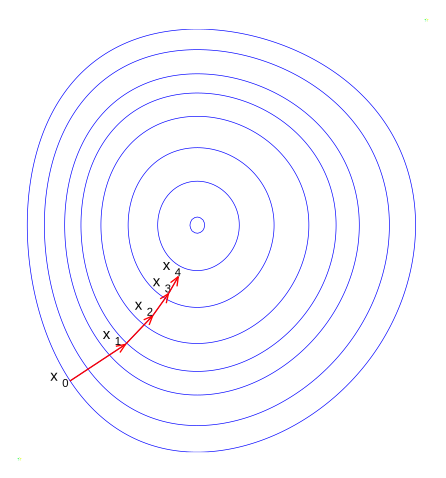
\includegraphics[width=0.4\textwidth]{images/gradient_descent}}
    \caption[Gradient descent]{Gradient descent \cite{pict}}
    \label{obr:gradient}
    \end{figure}
    
    
    \subsubsection{Stochastic gradient descent}
    
    During each gradient descent step, we need to go evaluate the gradient of the loss function over the whole dataset.
    This is usually not feasible for larger datasets. 
    
    We can exploit that usually the cost function $Q$ can be rewritten as a sum of costs for each data point.
    
    $$Q(\Theta) = \sum_{i=1}^n Q_i(\Theta)$$
    
    $Q_i(\Theta)$ denotes the cost function computed on only the $i$-th element. 
    Instead of performing the gradient step on the whole $Q$, 
    we can perform a gradient step for each $Q_i$. 

    $$\Theta^{t+1} = \Theta^t - \alpha \frac{\partial Q_i(\Theta^t)}{\partial \Theta^t} = \Theta^t - \alpha \nabla Q_(\Theta^t)$$
    
    For appropriate $\alpha$ we usually see a much faster convergence than for gradient descent.
    
    
    \subsection{Feed forward neural network}
    There is a lot of ways how to construct function $f_\theta$ that we want to optimize. 
    One of the most popular ones is roughly inspired by the human brain and is called a \textit{feed forward neural network}.
    
    Neural network consists of small interconnected computational units (neurons) that are usually organized into a layers.
    Each unit takes some inputs, based on them produces an output and sends it to other units. 
    In a feed forward neural network, the signal is always moving forward,
    hence unit on the $k$-th layer can only take it's input from previous layers \cite{Goodfellow-et-al-2016}.
    
    By adjusting the connections and theirs strengths, the network can learn to produce a specific output for a specific input.
    
    Simple neural network can be seen on an image \ref{obr:siet}.
    
    \begin{figure}[h]
    \centerline{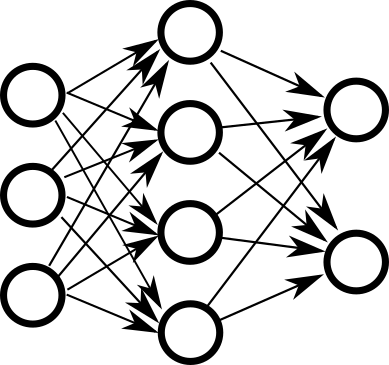
\includegraphics[width=0.4\textwidth]{images/neural_network}}
    \caption[Simple neural network with 2 layers, 3 inputs, 4 neurons and 2 outputs]{Simple neural network with 2 layers, 3 inputs, 4 neurons and 2 outputs\*} % redraw
    \label{obr:siet}
    \end{figure}
    
    The simplest realization of an unit is weighted sum and application of some function. 
    Formally the unit receives a vector of inputs $x$ and computes output $g(\sum_{i=1}^n w_i x_i)$, 
    where $w_i$ is a connection strength to the $i$-th input.
    This one unit can be viewed as a simple one layer neural network with one output.
    
    Common realizations of function $g$ are: 
    \begin{itemize}
        \item logistic function $g(x) = \frac{1}{1+e^{-x}}$
        \item hyperbolic tangent $g(x)=\frac{e^x-e^{-x}}{e^x+e^{-x}}$
        \item relu $g(x) = \max(0,x)$ 
        \item leaky relu $g(x)=\log(1+\exp(x))$
    \end{itemize}
    
    One layer of such units can be compactly described thanks to matrix notation as
    $$y=g(X W)$$
    
    $X$ represents the input matrix (number of samples $n$ times number of features $k$) and $W$ is the matrix of weights (number of features $k$ times number of units $u$). Note that function $g$ is applied element-wise.
    
    The important observation is, that we can chain such layers to form a deeper neural network.
    
    $$y=g(g(X W_1) W_2)$$
    
    $W_1$ are weight of hidden neurons (first layer) and $W_2$ are weight of output neurons (second layer).
    There is no consensus in the community about how to count the layers. 
    For example the simple network on picture \ref{obr:siet} could be seen as a $3$ layer neural network,
    because it has input units, hidden units and output units.
    In this thesis we will use the number of matrices $W$ that crates the model.
    
    Neural networks represent very broad family of functions that can in fact approximate any other function \cite{cybenko1989approximation}.
    However, we need to train them first.
    
    \subsubsection{Back propagation}
    
    Back propagation is a method for efficient computation of the gradient of a neural network.
    It relies on the the fact, that neural networks are just a simple compositions of matrix multiplications and function applications. 
    It also relies on the fact, that functions used in the units are differentiable (almost everywhere).
    
    \textit{Back propagation} works in two parts, forward pass and backward pass.
    In the forward pass we feed to input to the network, compute activations of each layer and compute the final output.
    In the second pass, we make use of the chain rule and incrementally compute gradient with respect to each layer of the network.
    Then we use the gradient descent and optimize the parameters \cite{rumelhart1986david}.
    
    \* %example
    %Let's take for example the simple 2 layer neural network $y=g(g(X W_1) W_2)$ with the $L2$ loss. 
    %Let $h_1=g(X W_1)$. 
    %We need to compute $\frac{\partial Q(W_2)}{W_2} = \frac{E_y(g(h_1 W_2))}{\partial W_2}$. 
    %By using the chain rule we get 
    %$\frac{E_y(g(h_1 W_2))}{\partial W_2} = 
    %\frac{\partial E_y(\hat{y})}{\partial \hat{y}}\frac{\partial \hat{y}}{\partial W_2}$
    
\section{Classification}
    
    \subsection{SVM}
    
        \* % cite something
        Some basics of svm, example of classifier that does not use backprop.
    
    \subsection{Linear regression}
    
        simple example of neural network that is not trained with backprob, but with normal equations,  
        but can still be used to do backprob with regards to the input.
    
    \subsection{Neural networks}
    
        some more information about neural network training for classification

    
\section{Word and sentence representation}

    \subsection{Motivation}
    
    In order to apply machine learning techniques to a text classification, 
    we need to represent the text in a machine learning friendly way.
    Most machine learning algorithms expect the input in a form of vectors of numbers. 
    
    Because of this, we need a system to translate string sentences $s$ into vectors of numbers $e$.
    Such vector is usually called an embedding. 
    
    In  other words, we need to project words and sentences into a vector space.
    
    
    \subsection{Local representation}
    
    The simplest vector space is based on a local representation.
    In this representation, we use a vector space with $|D|$ dimensions, one for each word in the vocabulary.
    Value $v_i$ at the $i$-th position of the vector $v$ corresponds to a presence or an absence of the $i$-th words from the vocabulary, $D_i$.
    Note, that $|D|$ in real applications easily exceeds $100\,000$ or even $1\,000\,000$.
    This may make this representation unusable for some applications (classification with SVM).
    
    One of the simplest local representation is called a \textit{bag of words} (BOW). 
    In this representation, values in vectors are binary, where $1$ means that the word was present in the sentence and $0$ means it was not.
    This can also be viewed as a simple one hot encoding.
    Optionally we can extend this to a term vector, where the number is not binary, but it express the real count of given word in the sentence.
    
    Let's look at our example corpus. 
    Our vector space would have $11$ dimensions and the first sentence would be represented as a vector
    $e = (1, 0, 0, 1, 1, 1, 1, 0, 0, 0, 0)$.
    
    This representation allows for simple sentence comparison. 
    Two sentences $s_1$ and $s_2$ can be compared via comparing cosine similarity of their BOW embeddings $e_1$ and $e_2$.
    $$\mathrm{sim}(s_1, s_2) = \mathrm{sim}(e_1, e_2) = \frac{e_1 e_2}{||e_1||.||e_2||}$$
    
    For technical reasons we can also define a cosine distance. 
    $$\mathrm{dist}(s_1, s_2) = \mathrm{dist}(e_1, e_2) = 1- \mathrm{sim}(e_1, e_2) = 1 - \frac{e_1 e_2}{||e_1||.||e_2||}$$
    
    However this representation does not consider, that two words can be similar, even though they are not the same.
    For example words \texttt{nice} and \texttt{good} are consider completely different, even though they are not. 
    
    Second problem is, that this representation forgets the initial ordering of the words.
    This can be partially solved by using bigrams.
    
    Third problem is, that this representation assigns the same weight to each word.
    The fact that two sentences both has a meaningless word \texttt{a} has the same effect on the similarity as 
    if they both have word \texttt{bad}. 
    This problem is partially solved by introducing term weights.
    
    
    \subsubsection{Term-weighting schemes}
    
    To emphasize that some words in the corpus are more important than other we introduce a term-weighting schemes. 
    The idea is, that words like prepositions (\texttt{a}, \texttt{an}) and other words that are not very informative or redundant (\texttt{is}, \texttt{do}, \texttt{by}) should have smaller weights. 
    In practice, a list of \textit{stop words} is used to completely filter such words.
    
    Also words, that are to common in the dataset should have lower weights.
    If each sample is about a dog, we probably do not care about the word \texttt{dog}, because it is somehow redundant.
    
    However words, that appear multiple times in a sentence are probably important for this sentence and should have higher weights.
    
    Based on these two observations, a number of Term-weighting schemes was proposed \cite{salton1988term}.
    A Term-weighting schemes assign a weight to a word $w$ in a sentence $s$ as term weight $t_{w,s}$.
    These weights usually consists of two parts, \emph{term frequency} and \emph{inverse document frequency}. 
    
    \emph{Term frequency}, $\mathrm{TF}_{w,s}$, part reflects how important is word $w$ for sentence $s$.
    Common choices are:
    \begin{itemize}
        \item $\mathrm{sign}(\mathrm{tf}_{w,s})$, binary presence of the word in sentence. Also known as BOW.
        \item $\mathrm{tf}_{w,s}$, number of appearances.
        \item $\frac{\mathrm{tf}_{w,s}}{|s|}$, number of appearances normalized by length of the sentence.
        \item $1+\log(\mathrm{tf}_{w,s})$.
    \end{itemize}
    
    \emph{Inverse document frequency}, $\mathrm{IDF_w}$, part reflects how important is the word $w$ for the whole corpus.
    Common choices are:
    \begin{itemize}
        \item $1$, unary.
        \item $\log \left(\frac{N}{n_w} \right)$, inverse document frequency.
        \item $\log \left( 1+\frac{N}{n_w} \right)$, smoothed inverse document frequency.
        \item $\log \left( \frac{max_{w'} n_{w'}}{n_w} \right)$, max inverse document frequency.
        \item $\log \left(\frac{N-n_w}{n_w} \right)$, probabilistic inverse document frequency.
    \end{itemize}

    Combination of such weight is called TFIDF.
    Note, that these choices for $\mathrm{TF}_{w,s}$ and $\mathrm{IDF}_{w,s}$ have probabilistically grounded \cite{aizawa2003information}. %information perspective on tfidf
    
    Another popular weighting scheme that is usually used in document retrieval is $\mathrm{BM_{25}}$. 
    
    $$\mathrm{BM}_{25~w,s} = \log \left(\frac{N-n_w+0.5}{n_w + 0.5}\right)    \frac{\mathrm{tf}_{w,s} (1.2 + 1)}{\mathrm{tf}_{w,s} + 1.2  \left(1 - 0.75 + 0.75 \cdot \frac{N}{\text{avgdl}}\right)}$$
    
    This representation performs better than BOW and usually works the best for large documents in document retrieval \cite{li2014semantic}.
    
    Term weight can help to describe that different words, have different importance.
    However, they still can not take into account, that two different words should have similar representation.
    
    
    \subsection{Distributed representation}
    
    To address the problem of high dimensionality and to allow different words to have high cosine similarity, we employ distributed representation.
    In this representation, dimensions do not correspond directly to words, but rather to some features of these words.
    In this representation the ''meaning`` of the word is split across multiple dimensions.
    We can view each dimension as if it holds some form of an abstract meaning \cite{le2014distributed}. 
    
    Simple but unrelated example of distributed representation is a binary representation of a number.
    
    To acquire a distributed representation, algorithms often make use of the Distributional hypothesis.
    \* % fix, that it is supervised vs unsupervised

    \subsubsection{Distributional hypothesis}
    
    Distributional hypothesis states, that words that appear in similar contexts tend to have similar meaning,
    even though they do not appear directly together \cite{harris1954distributional} \cite{Rubenstein:1965:CCS:365628.365657}. % distributional hypothesis 
    For example we can exchange words \texttt{dog} and \texttt{cat} in each sentence in our example corpus \ref{tab:example:dataset}
    and all sentences will still make sense. 
    The positive correlation between the words appeared in similar contexts and words having similar meaning was in fact empirically confirmed.
    
    Because of this, distributional hypothesis is used as a foundation for a lot of methods that try to capture the word semantic similarity \cite{rubenstein1965contextual}. 

    \subsection{Prediction based distributed representation}
    
    Number of researchers used neural networks to create a good, dense, distributed word representations \cite{pennington2014glove} \cite{DBLP:conf/icml/LeM14} \cite{rong2014word2vec}. % slovne vektory, some word2vec shit, glove word vectors
    These representations are also commonly called \emph{neural embeddings}.
    We will call these representations as \emph{word vectors}.
    Word vectors proved to be very useful in broad range of natural language processing tasks. 
    
    Moreover, they manifest interesting algebraic properties. 
    
    $$v(king) - v(man) + v(woman) = v(queen)$$
    $$v(better) - v(good) + v(small) = v(smaller)$$
    
    $v$ denotes a the word vector for given word.
    
    There are two main approaches for training word vectors with neural networks: skip-gram model and continuous bag of words model.
    
    Based on an embedding of an input word $x$, the \textit{skip-gram model} predicts words from $x$'s context.
    
    On the other hand, the \textit{continuous bag of words model} tries to predict the word based on it's context.
    
    These methods can be computationally intensive, and they require a lot of training data. 
    Moreover their training usually requires a lot of well chosen hyper-parameters ind tricks \cite{DBLP:journals/corr/MikolovSCCD13}. % podvzorkovanie
    

    \subsection{Count based distributed representation}
    \* % TODO write this better, find citations.
    
    Count based methods create coocurence matrix and factorize it it to eliminate noise, 
    what is left should reflect the meaning. 
    
    Different approach is a latent dirichlet allocation.
    
    Explicit semantic analysis
    Latent semantic analysis
    Hierarchical Dirichlet process
    Non-negative matrix factorization
    
    
    \subsubsection{Latent semantic analysis}
    
    During this thesis we consider the \emph{latent semantic indexing} (LSI) to be the same as \emph{latent semantic analysis} (LSA).
    For simplicity, we will refer only to the LSA.
    
    \emph{Latent semantic analysis} is one of the standard approaches to identify hidden variables describing the data.
    
    In the context of natural language classification it extracts and infers relations of expected contextual usage of words in documents.
    It does so without any humanly constructed dictionaries, knowledge bases, semantic networks, grammars or syntactic parsers.
    
    LSA starts with a coocurence matrix $M'$. 
    Each cell $M'_{i,j}$ of this matrix contains number representing the frequency with  which  the  word $D_i$ appears in the document $d_j$.
    Afterwards each cell entry is weighted by a function that expresses both the word's importance in the particular document and the word importance in the general corpus.
    A weighting scheme such as TFIDF can be used.
    We denote the reweighted matrix $M$. 
    
    Next, LSA applies singular value decomposition (SVD) to the matrix.
    In principle, SVD achieves a two-mode factor analysis and positions both terms and documents in a single space defined over the extracted dimensions.
    In case a different matrix factorization is used such as non negative matrix factorization, we would arrive to probabilistic latent semantic analysis.
    
    SVD breaks down the document matrix $M$ into three matrices $U$, $\Sigma$, $V$, 
    such that $M=U \Sigma V^T$ \cite{papadimitriou2000latent} % interpretation of lsa, steal some introduction 
    \cite{deerwester1990indexing} % first lsi/lsa?
    \cite{maas2011learning} % lda, vector space model
    \cite{wiemer2004latent} % Latent semantic analysis
    \cite{landauer1998introduction}. % introduction to lsa

    $U$ and $V$ are orthogonal matrices and $\Sigma$ is a diagonal matrix.
    
    {$$
\begin{matrix} 
 M &  ~~ U & \Sigma & V^T \\
 \textbf{t}_j^T &  & &  \\
 \downarrow &  & &  \\
(\textbf{d}_i) \rightarrow 
\begin{bmatrix}
x_{1,1} \dots  x_{1,n} \\
\vdots ~~~  \ddots ~~~ \vdots \\
x_{i,1} \dots  x_{i,n} \\
\vdots ~~~ \ddots ~~~ \vdots \\
x_{m,1} \dots  x_{m,n} \\
\end{bmatrix}
=
&
\textbf{u}_i \rightarrow
\begin{bmatrix} 
\begin{bmatrix} & \textbf{u}_1 & \end{bmatrix} \\
\vdots \\
\begin{bmatrix} & \textbf{u}_l & \end{bmatrix}
\end{bmatrix}
&
\cdot
\begin{bmatrix} 
\sigma_1 \dots ~~~ 0 \\
\vdots ~~~ \ddots  \vdots \\
0  \dots  \sigma_l \\
\end{bmatrix}
&
\cdot
\begin{bmatrix} 
\begin{bmatrix} \, \\ \, \\ \textbf{v}_1 \\ \, \\ \,\end{bmatrix} 
\dots
\begin{bmatrix} \, \\ \, \\ \textbf{v}_l \\ \, \\ \, \end{bmatrix}
\end{bmatrix}
\end{matrix}
$$}

    $U$ describes the original row entities (words) as vectors of derived orthogonal  factor values. 
    $V$ describes the original column entities (documents) in the same way.
    $\Sigma$ containing scaling values such that when the three components are matrix multiplied, the original matrix is reconstructed.

    It was shown that any matrix can be decomposed perfectly in a such way, using no more factors than the smallest dimension of the original matrix.
    
    Moreover we can construct a reduced rand approximation by setting all but the $k$ biggest entries in $\Sigma$ to zero. 
    This effectively reduces the number of columns of $U$ to $k$ and similarly number of rows of $V^T$.
    The thesis behind LSI is that those less important dimensions correspond to “noise” due to word-choice variability.
    
    Note that due to this reduction we inevitably loose some of the information. 
    We can see this as forgetting some of the less represented words.

    An interesting property of SVD is that the generated approximation is the closest matrix of its rank to the original in the least-squares sense.

    In practice we computing the full SVD decomposition would be time an memory unfeasible.
    Because of that, we directly compute the lower rank approximation with $k$ dimensions,
    such that $M \simeq U_k \Sigma V_k^T$ \cite{halko2011finding}. %fast svd
    Moreover, we do not even need to have access to the full matrix $M$ and we can compute the decomposition in an incremental manner \cite{brand2006fast}. % incremental svd
    
    Not only we can add incrementally adjust the decomposition when adding a new document into the corpus, we can remove the document as well.
    Incremental SVD could in theory be used in the stochastic gradient descent setting.
    
    From now on, we drop the subscript $k$ and matrices $U$, $\Sigma$ and $V$ in the later text are assumed to have only $k$ dimensions.
    
    
    \subsubsection{LSA for classification}
    
    In context of document classification, we first construct our vocabulary $D$ from our training data. 
    We can filter out words that we know, are not relevant, or that have only a few appearances in the corpus.
    
    Now we can transform sentences into their BOW representation.
    Afterwards, we compute all necessary statistics required by our chosen weighting scheme. 
    In case of TFIDF, we compute the number of appearances of each word in our text $n_w$. 
    This can be done efficiently by making use of fast matrix operations and libraries implementing linear algebra.
    
    Having these statistics, we can reweigh all words in sentences according to them and construct the term matrix $M$.
    
    Then we factorize $M$ an compute the matrices $U_k$, $\Sigma$, $V_k$. 
    In theory, we could directly read the document embeddings $v$ from the matrix $V$.
    For practical purposes, the matrix $V_k$ is usually not stored and sometimes not even computed. 
    
    To compute the embedding, we take the document term vector $d_i$ and employ a relationship $$d_i^T = U \Sigma v_i^T$$
    
    Because $U$ is orthogonal and $\Sigma$ is diagonal, we get
    
    $$\Sigma^{-1} U^T d_i^T = v_i^T $$

    $$v_i = d_i U \Sigma^{-1} $$
    
    Note, that $\Sigma^-1$ is easy to compute, becaues $\Sigma$ is a diagonal. 
    We just need to invert each number on the diagonal.  
    
    As was shown experimentally shown in my bachelor thesis \* % cite batchelor thesis 
    and by other researchers, $\Sigma$ may not properly 
    
    Matrix of such $v_i$ are then considered to be document features and are used as an input ($X$) to some classifier.
    
    Important part is, that we can we can compute the such embedding even for unseen documents.
    The problem is, that we have to filter all words that are not present in $D$. 
    However, because this method is fully unsupervised, we can make use of any unlabeled data (documents, that do no have known label).
    
    \subsubsection{LSA pitfalls}

    Even though LSA was shown to perform well in document retrieval applications and it can capture some basic semantic properties of words,
    it has certain limitations when applied to classification tasks. 
    
    The problem is, that LSA does not incorporate the the information about document classes. 
    It finds the most representative features and not the most discriminative ones.
    In other words, it finds embedding that is the best for reconstructing the documents.
    Because of that, infrequent words that have high discriminatory power (are important for the task), may be filtered out.
    
    For example, LSA computed on our example corpus \ref{tab:example:dataset} would focus on capturing the words \texttt{a}, \texttt{is}, \texttt{dog} and \texttt{cat},
    event htough they are completely irrelevant to our prediction task.
    
    \* % TODO SVD Forsythe, Malcolm, Moller 1997  SVD 
    
    \subsection{Relationship of prediction and count based representations}
        
    LSA and other count based techniques used to be very popular alternative to local representations.
    However after the raise of neural networks, they were soon overshadowed by neural word embeddings.
    
    Prediction based models achieved much better performance across multiple word relatedness tasks, categorization tasks, synonyms tasks and analogy tasks \cite{baroni2014don}. % do not count, predict
    
    During these evaluations, they obtained the word representations by training on a big monolingual dataset, like wikipedia.
    Then they used a prepared pairs of related words (synonyms or words from the same category) and tested,
    how similar are the vector representations of related words. 
    In other words, how well the word vector similarity correlates with the actual relatedness. 
    Count based methods achieved Pearson correlation coefficient $0.74$ and were outperformed by prediction based methods which achieved $0.84$ \cite{baroni2014don}.
    
    This, and the hype around neural network lead to recent extreme popularity of prediction based embeddings,
    even though they were much less understood and less ''mathematically grounded``.
    
    However, later it was shown, that these two approaches are in fact very similar.
    It was proven, that a prediction based model skip-gram with negative-sampling (SGNS) 
    is implicitly factorizing a word-context matrix,
    whose cells are the point-wise mutual information (PMI) of the respective word and context pairs, 
    shifted by a global constant \cite{levy2014neural}. % word2vec as matrix factorization 
    
    These results suggest, that these two approaches are somehow equivalent and with proper weights the LSA should achieve similar results as skip-gram model. 
    However in practice, this was not the case.
    
    Soon it was found, that the effectiveness of the neural embeddings is due to their numerous hyperparameters.
    These models require a lot of hyperparameters, that can not be learned and need to be set up manually,
    or through excessive search.
    On the other hand, count based models usually do not require a lot of parameters, besides the number of dimensions of the resulting embedding. 
    
    Levy et al. \cite{levy2015improving} % word2vec hacks in lsi
    showed, that much  of  the  performance  gains  of  neural embeddings  are  due  to  certain  system design  choices and hyperparameters, rather than the embedding algorithms themselves. 
    Furthermore they showed that traditional (count based) distributional models, 
    can also benefit from such hyperparameters and design choices.
    
    After incorporating these insights into the count based methods, 
    they observed mostly local or insignificant performance differences between these approaches.
    
    Note, that these experiments were done on a large bodies of text like English Wikipedia.   
    On small datasets it was empirically shown, that count based methods actually outperform the neural networks.\cite{altszyler2016comparative}. % lsa vs word2vec on samall corpora
    
    \* \cite{naili2017comparative} % wrf is this? some comparison

\section{Other approached for document classification}
    
    Recurrent neural networks,
    Character based recurent neural networs, 

\* %\cite{manning2008introduction} introduction to information retrieval}


\chapter{Similar work}
    \section{LSI with class knowledge}
        \subsection{Supervised LSI}
            \cite{sun2004supervised} %supervised lsi, discriminative basis

        \subsection{Sprinkling}
            \cite{chakraborti2007supervised} % Sprinkling
        
        \subsection{Supervised weights} \label{sec:supervised:weights}
            \cite{wu2017balancing} % word weights, TODO read
            \cite{ji2013discriminative} % TF KLD
            \cite{deng2014study} % supervised weights
            \cite{lan2009supervised} % supervised weights for text categorization

    
    \section{SVD in neural networks}
        \subsection{SVD as structured layer} 
            \cite{ionescu2015training} % svd in neural networks

    
\chapter{Our approach}
    
    In this chapter we describe our motivations, the actual design of our approach and implementations details.
    
    \section{Goals and motivation}
    
    \* %TODO introduce minimal amount of hyperparameters,
    \* %TODO be able to get some insight and interpretability out of the model,

    In LSA, the SVD will inevitably throw away some information. 
    This is due the dimensionality reduction that it performs.
    The problem is, that this information may be vital to the classification task. 
    It is clear, that we need to introduce some form of supervision, that happens before the SVD.
    
    This is done to some extend by the supervised word weights described in section \ref{sec:supervised:weights}. 
    However, we consider this supervision rather weak, as it only computes simple statistics over words and labels.
    
    We would like to incorporate some form of direct supervision, that can directly affect which words are remembered by the SVD and which are thrown away.
    
    Because of the supervised weights, we know that supervision helps. 
    The only problem is, how to achieve it. 
    Here we take the inspiration from neural networks, and the insight that we can easily optimize parameters of rather complex system, as long as each part of this system is differentiable. 
    
    \section{Design}
    
    First recall how does the original LSA works in context of document classification.
    We start with a sentence $s_i$. We represent it as a sparse vector, a bag of words vector $d_i'$. 
    With some weighting scheme we transform it into a term vector $d_i$.
    Afterwards we compute the lower dimensional embedding of the document $v_i = d_i U$. 
    
    Finally we use these embeddings $v_i$ as features $x_i$ that are an input the the classifier (logistic regression, neural network, SVM).
    This classifier predicts some labels $\hat{y}$ that can be compared to
    the true labels $y$.
    
    Our contribution is to introduce another layer of reweighting. 
    Instead of using the term vector $d_i$, we introduce weights $w'$ and use reweighted vector as $d_i \circ w'$.
    Recall, that $\circ$ means Hadamard product (pointwise multiplication).
    This is equivalent to multiplying the vector $d_i$ by diagonal matrix with diagonal $w'$.
    
    This means, we do not perform the SVD decomposition on the matrix $M$, 
    but on the reweighted version $M \circ w'$. 
    Here we employ a few conventions from popular linear algebra library NumPy \cite{oliphant2006guide}, 
    where such operation is automatically broadcasted through the matrix.
    
    We initialize the $w'$ to be a vector of ones. 
    This effectively does not change the matrix at first.
    Now we are interested, in finding the best $w'$. 
    
    Recall, that for fixed decomposition $M\circ w'= U\Sigma V^T$ and some classifier $c$ (like a neural network),
    we compute $\hat{y} = g(M \circ w' U)$.
    We want to optimize $w'$ to minimize some error $E_y(\hat{y})$.
    The only question is, how to do it?
    
    The natural candidate is the gradient descent. 
    However to use it, we need to be able to compute the gradient of error with regards to the weights $\frac{\partial E_y(\hat{y})}{\partial w'}$
    
    \subsection{Gradient computation}
    
    To compute the gradient efficiently, we recall the back-propagation trick described in section \ref{sec:backprop}.
    We can compute the derivation $\frac{\partial E_y(\hat{y})}{\partial w'}$ thanks to the chain rule
    
    \begin{align}
    \frac{\partial E_y(\hat{y})}{\partial w'} = \frac{\partial E_y(\hat{y})}{\partial \hat{y}} \frac{\partial c(x)}{\partial x} \frac{\partial x}{\partial d}
    \end{align}
    
    To compute the derivation $\frac{\partial E_y(\hat{y})}{\partial w'} = \frac{\partial E_y(\hat{y})}{\partial \hat{y}} \frac{\partial c(x)}{\partial x} \frac{\partial x}{\partial d}$ we realize,
    that each part of this expression is easy to calculate.
    
    The first part of this expression is a function dependent on the chosen error function. 
    For L2 error we get 
    $\frac{\partial E_y(\hat{y})}{\partial \hat{y}} = \frac{\partial \frac{1}{2}(\hat{y}-y)^2}{\partial \hat{y}} = \hat{y}-y$
    
    The second part is dependent on the classifier that we use. 
    In case we use logistic regression $\hat{y} = \sigma(x \Theta + b)$, the expression becomes
    $\frac{\partial c(x)}{\partial x} = \hat{y} (1-\hat{y}) \Theta$
    Note, that it is easy to compute this expression even for more complicated classifiers. 
    Some libraries can even compute this automatically \cite{tensorflow2015-whitepaper}.
    However we still need that the classifier is differentiable, so we can not easily use SVM. 
    
    The third and last part is tied to the computation of LSA embedding.
    Because $x = d \circ w' U$, we can compute 
    $\frac{\partial x}{\partial d} = d U$ \* % TODO fix this math stuff
    
    Once we computed the gradient, we need to decide on the the optimization routine we employ.
    
    \subsection{Optimization routine}
    
    We want to perform the gradient step $w' = w' - \frac{\partial E_y(\hat{y})}{\partial w'}$. 
    However this changes the input to the SVD and we should recompute the decomposition as well. 
    However it is not clear, how often we want to recompute the SVD and how often (and how much) we want to retrain the classifier.
    We propose two main approaches inspired by neural network training and by 
    expectation minimization algorithm. \* % TODO cite something
    
    Our model can be broken down into three parts: weighting, decomposition and classification.
    We will denote the weighting part as $W$, the decomposition part as $S$ (SVD) and the classification part as $C$.
    Also as this parts are going to be updated through the time, we will denote them with superscripts $W^t$, referring to $W$ at time $t$.
    
    \* %todo, code EM algo (optimize w' while possible, then recompute LSA)
    
    \subsubsection{Batch gradient descent}
    In this setting, 
    
    
    \subsubsection{Stochastic gradient descent}
    
    We take the inspiration from stochastic gradient descent for neural networks.
    Instead of computing the full gradient, we just compute the gradient related to one example $\frac{\partial E_{y_i}(\hat{y_i})}{\partial w'}$
    Because the document vector $d_i$ is sparse, we will only update a few values from $w'$, 
    hence we can easily update part $W$.

    Because we updated $w'$, the entry in matrix $M$ corresponding to the document $d_i$ changed.
    We know, that SVD can be build incrementally and that we can add new documents to the matrix $M$ \cite{brand2006fast}.
    We just use the adding routine and add the new representation $d_i w'^{t+1}$ to the decomposition.
    Because we changed the reweighed document and the the decomposition matrices,
    the embedding of this document also changed to 
    $x_i^{t+1} = v_i^{t+1} = d_i w'^{t+1} U^{t+1}$
    
    We update $C$ in the similar manner.
    We just perform the stochastic gradient step for example $x_i^{t+1}$ and threat it as a new example in the dataset.
    
    \section{Implementation}
        
        In the implementation
        \cite{bird2009natural} % nlp in python
        \cite{oliphant2006guide} % numpy
        
        Our implementation is available on github \*% add link
        
        \subsection{Gensim lsa}
        \cite{rehurek_lrec}
        \* % TODO Intro about gensim
        \* % TODO cite the fast lsa in gensim
        \* % TODO, cite other important objects we use (dictionaries, sparse corpus), weights, word2 vec implementation
        
        \subsection{Scikit-learn}
        \cite{sklearn_api},
        \cite{scikit-learn}
        \* % TODO classifiers
        \* % TODO 
        

        \subsection{Tensorflow for clasifier?}
        \* % do i want to implement the clasifier in tf?
        \* % note about computing the gradient authomaticaly,
        \* % discuss not used because of fast svd is not there.
    
        \subsection{Other used tools}
        \cite{perez2007ipython} %ipython
        \* % experiments, evaluation and development
        \* % cite python 
        \cite{hunter2007matplotlib} %matplotlib
        \cite{mckinney2010data}
        
        
        

\chapter{Experiments and evaluation}

    Performance
    
    Result analysis
    
    Weight analysis
    
    Transfer learning?

    \section{Classification datasets}
        \subsection{Datasets}
            \cite{conneau2017supervised} % datasets, benchmarks

    \section{Interpretability}
        \cite{ribeiro2016should} % explainability


